\section{Teoria generale dei limiti}

\begin{theorem}
	Teorema di struttura sui limiti. Limiti in funzione di altri limiti. In breve, TFAE:
	\begin{itemize}
		\item 	Cocompleteness,
		\item having coproducts and coequalizers,
		\item having coproducts and pushouts,
		\item having filtered colimits, finite coproducts and pushouts, and
		\item having filtered colimits, pushouts and an initial object.
		\item ...?
	\end{itemize}
	Kelly closure of a class of colimits
\end{theorem}
Il teorema di struttura è molto utile nel decomporre un limite o colimite di forma complessa in un co/equalizzatore di mappe tra co/prodotti, o in un prodotto fibrato o somma amalgamata, ad esempio...
\begin{example}
	Nella terminologia di \ref{ex_cat_turcasso}, si consideri come dominio di un diagramma un 3-turcasso \(\turk[3]\); un \emph{triqualizzatore} in una categoria \(\ctC\) è il limite di un diagramma \(D\colon \turk[3] \fun\ctC\), che quindi è della forma
	\[\xymatrix{X \ar[r]|-g \ar@<.5em>[r]^-f \ar@<-.5em>[r]_-h& Y}\]
	per tre frecce parallele \(f,g,h\colon X\to Y\) in \(\ctC\). La punta del cono limite è un oggetto \(\eq_3(f,g,h)\in\ctC_0\), con una freccia \(e_3 \colon \eq_3(f,g,h) \to X\) e la proprietà che
	\begin{itemize}
		\item \(f\cmp e_3 = g\cmp e_3 = h\cmp e_3\);
		\item per ogni \(z \colon Z \to X\) tale che \(f\cmp z = g\cmp z = h\cmp z\), esiste un'unica \(\bar z \colon Z \to \eq_3(f,g,h)\) tale che \(z = e_3\cmp \bar z\).
	\end{itemize}
	In virtù di \ref{}, il triqualizzatore di \(f,g,h\) è esprimibile come \emph{equa}lizzatore di una coppia di frecce in \(\ctC\), precisamente si ha
	\[\eq_3(f,g,h) \cong \eq\Bigl(
		\xymatrix@C=2cm{
			X\times Y \ar@<.3em>[r]^-{\bkt{\pi_Y,\pi_Y,\pi_Y}}\ar@<-.3em>[r]_{\bkt{f\cmp\pi_X,g\cmp\pi_X,h\cmp\pi_X}} & Y\times Y \times Y
		}
		\Bigr)\]
	dove come di consueto indichiamo \(\bkt{u,v,w}\) la freccia \(\pair u{\pair vw}=\pair{\pair uv}w\).

	C'è però una maniera più diretta di ottenerlo mediante la combinazione di due equalizzatori e di un prodotto fibrato: consideriamo il diagramma
	% https://q.uiver.app/#q=WzAsNixbMSwxLCJYIl0sWzIsMSwiWSJdLFswLDAsIlQiXSxbMSwwLCJFJyJdLFswLDEsIkUiXSxbMSwyLCJZIl0sWzIsMywicCJdLFszLDAsImVfMiJdLFs0LDAsImVfMSIsMl0sWzIsNCwicSIsMl0sWzAsMSwiZiIsMCx7Im9mZnNldCI6LTF9XSxbMCw1LCJoIiwwLHsib2Zmc2V0IjotMX1dLFswLDUsImciLDIseyJvZmZzZXQiOjF9XSxbMCwxLCJnIiwyLHsib2Zmc2V0IjoxfV0sWzIsMCwiciIsMV1d
	\[\begin{tikzcd}[ampersand replacement=\&]
			T=\pull E{E'}X \& {E'} \\
			E \& X \& Y \\
			\& Y
			\arrow["p", from=1-1, to=1-2]
			\arrow["q"', from=1-1, to=2-1]
			\arrow["r"{description}, from=1-1, to=2-2]
			\arrow["{e_2}", from=1-2, to=2-2]
			\arrow["{e_1}"', from=2-1, to=2-2]
			\arrow["f", shift left, from=2-2, to=2-3]
			\arrow["g"', shift right, from=2-2, to=2-3]
			\arrow["h", shift left, from=2-2, to=3-2]
			\arrow["g"', shift right, from=2-2, to=3-2]
		\end{tikzcd}\]
	dove \((E,e_1)\) è l'equalizzatore della coppia \((f,g)\), e \((E',e_2)\) è l'equalizzatore della coppia \((g,h)\), e il quadrato è un prodotto fibrato. Dimostriamo che \((T,r)\), dove \(r = e_1\cmp q=e_2\cmp p\) è il triqualizzatore di \((f,g,h)\): innanzitutto,
	\begin{align*}
		\underline{f\cmp r} & = f\cmp e_1\cmp q     \\
		                    & =g\cmp e_1\cmp q      \\
		                    & =\underline{g\cmp r}  \\
		                    & =g\cmp e_2\cmp p      \\
		                    & =h\cmp e_2\cmp p      \\
		                    & =\underline{h\cmp r}.
	\end{align*}
	Se ora supponiamo che esista \(z\colon Z \to X\) tale che \(f\cmp z=g\cmp z=h\cmp z\), \(z\) equalizza sia la coppia \((f,g)\) (e allora \(z=e_1\cmp \bar z_1\) per un'unica \(z_1\)) sia la coppia \((g,h)\) (e allora \(z=e_2\cmp \bar z_2\) per un'unica \(z_2\)); quindi
	\[e_1\cmp \bar z_1=z=e_2\cmp \bar z_2\]
	cosa che implica che la coppia \(\pair{z_1}{z_2} \colon Z \to E\times E'\) fattorizzi lungo il prodotto fibrato \(\pull E{E'}X=T\). La costruzione è rappresentata, un passaggio alla volta, nel diagramma in Figura \ref{fig_triqual_construzia}.
\end{example}
\begin{figure}
	\begin{minipage}{0.33\textwidth}
		% https://q.uiver.app/#q=WzAsMyxbMSwwLCJYIl0sWzIsMCwiWSJdLFswLDAsIkUiXSxbMiwwLCJlXzEiLDJdLFswLDEsImYiLDAseyJvZmZzZXQiOi0xfV0sWzAsMSwiZyIsMix7Im9mZnNldCI6MX1dXQ==
		\[\begin{tikzcd}[ampersand replacement=\&]
				E \& X \& Y
				\arrow["{e_1}"', from=1-1, to=1-2]
				\arrow["f", shift left, from=1-2, to=1-3]
				\arrow["g"', shift right, from=1-2, to=1-3]
			\end{tikzcd}\]
	\end{minipage}%
	\begin{minipage}{0.33\textwidth}
		% https://q.uiver.app/#q=WzAsNSxbMSwxLCJYIl0sWzIsMSwiWSJdLFswLDEsIkUiXSxbMSwwLCJFJyJdLFsxLDIsIlkiXSxbMiwwLCJlXzEiLDIseyJjb2xvdXIiOlswLDAsNjldfSxbMCwwLDY5LDFdXSxbMCwxLCJmIiwwLHsib2Zmc2V0IjotMSwiY29sb3VyIjpbMCwwLDY5XX0sWzAsMCw2OSwxXV0sWzAsMSwiZyIsMix7Im9mZnNldCI6MSwiY29sb3VyIjpbMCwwLDY5XX0sWzAsMCw2OSwxXV0sWzMsMF0sWzAsNCwiaCIsMCx7Im9mZnNldCI6LTF9XSxbMCw0LCJnIiwyLHsib2Zmc2V0IjoxfV1d
		\[\begin{tikzcd}[ampersand replacement=\&]
				\& {E'} \\
				\color{gray!50}E \& X \& \color{gray!50}Y \\
				\& Y
				\arrow[from=1-2, to=2-2]
				\arrow["{e_1}"', color=gray!50, from=2-1, to=2-2]
				\arrow["f", shift left, color=gray!50, from=2-2, to=2-3]
				\arrow["g"', shift right, color=gray!50, from=2-2, to=2-3]
				\arrow["h", shift left, from=2-2, to=3-2]
				\arrow["g"', shift right, from=2-2, to=3-2]
			\end{tikzcd}\]
	\end{minipage}%
	\begin{minipage}{0.33\textwidth}
		% https://q.uiver.app/#q=WzAsNixbMSwxLCJYIl0sWzIsMSwiWSJdLFswLDEsIkUiXSxbMSwwLCJFJyJdLFsxLDIsIlkiXSxbMCwwLCJUIl0sWzIsMCwiZV8xIiwyXSxbMCwxLCJmIiwwLHsib2Zmc2V0IjotMX1dLFswLDEsImciLDIseyJvZmZzZXQiOjF9XSxbMywwXSxbMCw0LCJoIiwwLHsib2Zmc2V0IjotMX1dLFswLDQsImciLDIseyJvZmZzZXQiOjF9XSxbNSwzXSxbNSwyXSxbNSwwLCIiLDEseyJzdHlsZSI6eyJuYW1lIjoiY29ybmVyIn19XV0=
		\[\begin{tikzcd}[ampersand replacement=\&]
				T \& {E'} \\
				E \& X \& \color{gray!50}Y \\
				\& \color{gray!50}Y
				\arrow[from=1-1, to=1-2]
				\arrow[from=1-1, to=2-1]
				\arrow["\lrcorner"{anchor=center, pos=0.125}, draw=none, from=1-1, to=2-2]
				\arrow[from=1-2, to=2-2]
				\arrow["{e_1}"', from=2-1, to=2-2]
				\arrow["f", color=gray!50,shift left, from=2-2, to=2-3]
				\arrow["g"', color=gray!50,shift right, from=2-2, to=2-3]
				\arrow["h", color=gray!50,shift left, from=2-2, to=3-2]
				\arrow["g"', color=gray!50,shift right, from=2-2, to=3-2]
			\end{tikzcd}\]
	\end{minipage}%
	% \begin{minipage}{0.5\textwidth}
	%   % https://q.uiver.app/#q=WzAsNyxbMiwyLCJYIl0sWzMsMiwiWSJdLFsxLDIsIkUiXSxbMiwxLCJFJyJdLFsyLDMsIlkiXSxbMSwxLCJUIl0sWzAsMCwiWiJdLFsyLDAsImVfMSIsMl0sWzAsMSwiZiIsMCx7Im9mZnNldCI6LTF9XSxbMCwxLCJnIiwyLHsib2Zmc2V0IjoxfV0sWzMsMF0sWzAsNCwiaCIsMCx7Im9mZnNldCI6LTF9XSxbMCw0LCJnIiwyLHsib2Zmc2V0IjoxfV0sWzUsM10sWzUsMl0sWzUsMCwiIiwxLHsic3R5bGUiOnsibmFtZSI6ImNvcm5lciJ9fV0sWzYsMywiel8yIiwwLHsiY3VydmUiOi0xfV0sWzYsMiwiel8xIiwyLHsiY3VydmUiOjF9XSxbNiw1LCJ6X1QiXV0=
	% \[\begin{tikzcd}[ampersand replacement=\&]
	% 	Z \\
	% 	\& T \& {E'} \\
	% 	\& E \& X \& Y \\
	% 	\&\& Y
	% 	\arrow["{z_T}", from=1-1, to=2-2]
	% 	\arrow["{z_2}", curve={height=-6pt}, from=1-1, to=2-3]
	% 	\arrow["{z_1}"', curve={height=6pt}, from=1-1, to=3-2]
	% 	\arrow[from=2-2, to=2-3]
	% 	\arrow[from=2-2, to=3-2]
	% 	\arrow["\lrcorner"{anchor=center, pos=0.125}, draw=none, from=2-2, to=3-3]
	% 	\arrow[from=2-3, to=3-3]
	% 	\arrow["{e_1}"', from=3-2, to=3-3]
	% 	\arrow["f", shift left, from=3-3, to=3-4]
	% 	\arrow["g"', shift right, from=3-3, to=3-4]
	% 	\arrow["h", shift left, from=3-3, to=4-3]
	% 	\arrow["g"', shift right, from=3-3, to=4-3]
	% \end{tikzcd}\]
	% \end{minipage}
	% \end{center}
	\caption{Costruzione del triqualizzatore di tre frecce \(f,g,h\) in termini di due equalizzatori e un prodotto fibrato. Si provi a dimostrare, per esercizio, il fatto ovvio che l'equalizzatore di \((f,g,g)\) coincide con l'equalizzatore di \((f,g)\).}
	\label{fig_triqual_construzia}
\end{figure}
\begin{example}
	Prodotto fibrato `ampio'
\end{example}
\begin{example}
	Somma amalgamata `ampia'
\end{example}

Def di limite mediante coni e coconi

rappresentabilità dei (co)limiti, esplicitamente.
Esempi.

Limiti e colimiti finiti, limiti e colimiti connessi.
Limiti cofiltrati, colimiti filtrati.
Limiti assoluti.

Funtorialità dei limiti e dei colimiti.

Invarianza dell'esistenza di co/limiti per equivalenza di categorie. Dualità scambiano limiti e colimiti.

Se \(\ctI\) e \(\ctJ\) sono equivalenti, \(\lim_\ctI D\cong\lim_\ctJ D\)?

thm: una categoria piccola (co)completa è un poset (Freyd).

\subsection{Mono, epi e limiti}
Epimorfismi come colimiti; monomorfismi come limiti. Chiusura degli epi per colimiti, chiusura dei mono per limiti. Coincidenza di alcune classi di mono-epi in presenza di co/limiti.

oss su coequalizzatori riflessivi; epi regolari; coppia nucleo, coppia conucleo; esattezza.
\begin{lemma}
	Sia \(\ctC\) una categoria. Ogni freccia \(m \colon A\to X\) tale che esista una coppia \(f,g \colon X \to Y\) di frecce parallele e un diagramma equalizzatore
	% https://q.uiver.app/#q=WzAsMyxbMCwwLCJBIl0sWzEsMCwiWCJdLFsyLDAsIlkiXSxbMSwyLCJmIiwwLHsib2Zmc2V0IjotMn1dLFsxLDIsImciLDIseyJvZmZzZXQiOjJ9XSxbMCwxLCJtIiwyXV0=
	\[\begin{tikzcd}[ampersand replacement=\&]
			A \& X \& Y
			\arrow["m"', from=1-1, to=1-2]
			\arrow["f", shift left=1, from=1-2, to=1-3]
			\arrow["g"', shift right=1, from=1-2, to=1-3]
		\end{tikzcd}\]
	è un mono. Dualmente, data \(p \colon Y\to B\), se esiste una simile coppia \(f,g \colon X \to Y\) e un diagramma coequalizzatore
	% https://q.uiver.app/#q=WzAsMyxbMCwwLCJYIl0sWzEsMCwiWSJdLFsyLDAsIkIiXSxbMCwxLCJmIiwwLHsib2Zmc2V0IjotMn1dLFswLDEsImciLDIseyJvZmZzZXQiOjJ9XSxbMSwyLCJxIiwyXV0=
	\[\begin{tikzcd}[ampersand replacement=\&]
			X \& Y \& B
			\arrow["f", shift left=1, from=1-1, to=1-2]
			\arrow["g"', shift right=1, from=1-1, to=1-2]
			\arrow["p"', from=1-2, to=1-3]
		\end{tikzcd}\]
	allora \(p\) è epi.
\end{lemma}
\begin{proof}
	Mostriamo il primo enunciato, il secondo è duale. Se \(m = \eq(f,g)\), e \(s,t \colon Z \to A\) sono tali che \(h = m \cmp s = m \cmp t\), allora abbiamo un diagramma
	% https://q.uiver.app/#q=WzAsNCxbMCwwLCJBIl0sWzEsMCwiWCJdLFsyLDAsIlkiXSxbMCwxLCJaIl0sWzAsMSwibSIsMl0sWzEsMiwiZiIsMCx7Im9mZnNldCI6LTF9XSxbMSwyLCJnIiwyLHsib2Zmc2V0IjoxfV0sWzMsMCwicyIsMCx7Im9mZnNldCI6LTF9XSxbMywwLCJ0IiwyLHsib2Zmc2V0IjoxfV0sWzMsMSwiaCIsMl1d
	\[\begin{tikzcd}[ampersand replacement=\&]
			A \& X \& Y \\
			Z
			\arrow["m"', from=1-1, to=1-2]
			\arrow["f", shift left, from=1-2, to=1-3]
			\arrow["g"', shift right, from=1-2, to=1-3]
			\arrow["s", shift left, from=2-1, to=1-1]
			\arrow["t"', shift right, from=2-1, to=1-1]
			\arrow["h"', from=2-1, to=1-2]
		\end{tikzcd}\]
	ma da ciò segue che \(u,v\) sono entrambe fattorizzazioni di \(h\)	attraverso il dominio \(\eq(f,g)_0\) di \(m\), e dalla proprietà universale deve seguire \(s=t\); dunque \(m\) è mono.
\end{proof}
Questo motiva la definizione seguente.
\begin{definition}[Epi e mono regolare]\label{def_epi_mono_regolari}\index{Monomorfismo!--- regolare}\index{Epimorfismo!--- regolare}
	Sia \(\ctC\) una	categoria.
	\begin{itemize}
		\item Se una freccia \(m \colon A \to X\) soddisfa l'ipotesi del lemma precedente, allora \(m\) è detta un \emph{mono regolare}.
		\item Dualmente, se una freccia \(p \colon Y \to B\)	soddisfa l'ipotesi del lemma precedente, allora \(p\) è detta un \emph{epi regolare}.
	\end{itemize}
\end{definition}
\begin{definition}[Categoria regolare]\label{def_cat_regolare}\index{Categoria!--- regolare}
	\color{red}
	Una categoria \(\ctC\) è detta \emph{regolare} se:
	\begin{itemize}
		\item ha tutti i prodotti finiti;
		\item ha tutti i coequalizzatori dei mono;
		\item gli epi sono stabili per pullback, ovvero il pullback di un epi lungo una qualsiasi freccia esiste ed è ancora un epi.
	\end{itemize}
\end{definition}
\begin{remark}
	La nozione di epi regolare è l'ultima	che ci serve per stabilire la `gerarchia delle frecce epi' (split epi \(\implies\)	epi regolare \(\implies\)	epi forte \(\implies\)	epi estremale, e analogamente per i mono). La situazione è descritta nella Figura \ref{fig_gerarchia} insieme ad una schematizzazione delle ipotesi a cui le inclusioni si possono invertire. Viene usata la notazione di \ref{}, cioè la definizione di classe \emph{ortogonale} a una classe di frecce, ma non si tratta di un concetto nuovo rispetto a \ref{mepi_forte}.\Todo{aggiungere le condizioni a cui classi di epi coincidono}
\end{remark}
\begin{figure}
	\begin{center}
		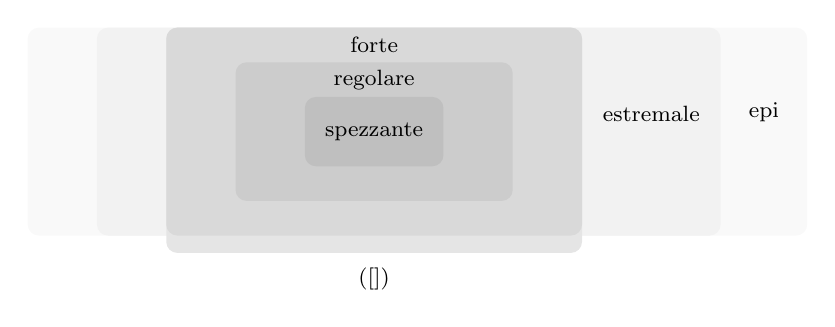
\begin{tikzpicture}[scale=1.1]
			% Outer to inner boxes
			\fill[gray!5,rounded corners] (-4,-1.2) rectangle (5,1.2);
			\node[font=\footnotesize,above] at (4.5,0.0) {epi};

			\fill[gray!10,rounded corners] (-3.2,-1.2) rectangle (4,1.2);
			\node[font=\footnotesize,above] at (3.2,0.0) {estremale};

			\fill[gray!20,rounded corners] (-2.4,-1.4) rectangle (2.4,1.2);
			\node[font=\footnotesize] at (0,-1.7) {$\lort(\Mono[\ctC])$};
			\fill[gray!30,rounded corners] (-2.4,-1.2) rectangle (2.4,1.2);
			\node[font=\footnotesize] at (0,1) {forte};

			\fill[gray!40,rounded corners] (-1.6,-0.8) rectangle (1.6,0.8);
			\node[font=\footnotesize] at (0,0.6) {regolare};

			\fill[gray!50,rounded corners] (-0.8,-0.4) rectangle (0.8,0.4);
			\node[font=\footnotesize] at (0,0) {spezzante};
		\end{tikzpicture}
	\end{center}
	\caption{Gerarchia delle classi di epimorfismi in una categoria \(\ctC\). Le inclusioni si possono invertire sotto le ipotesi indicate. Le classi \(\Epi[\ctC]^s\) degli epi forti di \ref{} e l'ortogonale sinistro \(\lort(\Mono[\ctC])\) sono `essenzialmente sempre' coincidenti nei casi reali, ma \ref{} è un controesempio. Ipotesi opportune su \(\ctC\) rovesciano alcune di queste inclusioni: \Todo{}}\label{fig_gerarchia}
\end{figure}
\subsection{Interazioni tra limiti e colimiti, completamenti}

Interazioni tra limiti e colimiti: commutatività di colimiti filtrati e limiti finiti, commutatività di colimiti setacciati e prodotti. Polinomi (`limiti e colimiti interagiscono per formare un polinomio')

completamenti (il completamento per iniziale è \(\ctC^\lhd\), quello per terminale è il cono destro \(\ctC^\rhd\); descrivere in casi semplici il completamento per prodotti e per coprodotti, gli altri sono più difficili...)

\subsection{Categorie piccolo-complete e piccolo-cocomplete}
